\documentclass[11pt]{article}
\usepackage[margin=1in]{geometry}
\usepackage{amsmath,amssymb,amsfonts}
\usepackage{amsthm,mathrsfs}
\usepackage{bm,bbm}
\usepackage{graphicx}
\usepackage{placeins}
\graphicspath{{figures/}}
\usepackage[colorlinks=true,linkcolor=blue,citecolor=blue,urlcolor=blue]{hyperref}

\theoremstyle{plain}
\newtheorem{theorem}{Theorem}[section]
\newtheorem{lemma}[theorem]{Lemma}
\newtheorem{proposition}[theorem]{Proposition}
\theoremstyle{remark}
\newtheorem{remark}[theorem]{Remark}
\numberwithin{equation}{section}

\title{The next generation matrix of the age- and location-stratified SEIR model\thanks{Parts of this manuscript were edited with the assistance of an AI tool (Claude Opus 5.5, Anthropic). The authors are solely responsible for all proofs and statements.}}
\author{Zhilan \and John \and Yuliya \and Ludmil}
\date{}

\begin{document}
\maketitle

\begin{abstract}
In the next generation matrix of the model of~\cite{2026Feng_Day_Glasser},
the columns of the immunologically naive and of the partially immune infected
carry different weights, $q_{s,p}$ and $q_{m,p}$. We show that its spectral
radius equals $\rho\left(A_1\operatorname{diag}(\bm g)\right)$, with
$A_1=\operatorname{diag}(\bm d_c)\,C\operatorname{diag}(\bm\psi_I\odot\bm q_s)$
independent of the vaccination rates and $g_p=y_p+r_pz_p$, $r_p=q_{m,p}/q_{s,p}$,
and we derive the formulas needed to minimize it over the vaccination rates.
\end{abstract}

\section{Setting}\label{sec-setting}

There are $m$ locations and $n$ age groups, $N=mn$, and the pair
$(i,j)$ is identified with $p=(i-1)n+j$; $I_i=\{(i-1)n+1,\ldots,in\}$. The
vaccination rates of the three doses are $\chi_{k,p}\ge 0$, $k=1,2,3$. We
consider the problem
\begin{equation}\label{problem}
\min\ \rho\left(\operatorname{NGM}(\bm\chi)\right)\quad\mbox{subject to}\quad
\sum_{p\in I_i}\sigma_{k,p}\chi_{k,p}=b_{k,i},\quad \chi_{k,p}\ge 0,\quad k=1,2,3,\ i=1:m,
\end{equation}
where $b_{k,i}\ge 0$ are the available doses of type $k$ at location $i$ and
$\sigma_{k,p}>0$ the sizes of the groups that receive them. At the disease
free equilibrium of~\cite{2026Feng_Day_Glasser} the fractions of susceptible,
vaccinated and partially immune people in group $p$ are $\widetilde s_p$,
$\pi_{1,p}\widetilde s_p$ and $\pi_{2,p}\pi_{1,p}\widetilde s_p$, where
\begin{equation}\label{pis}
\pi_{1,p}=\frac{\chi_{1,p}}{\omega_v+\varepsilon_2\chi_{2,p}},\quad
\pi_{2,p}=\frac{\varepsilon_2\chi_{2,p}}{\omega},\quad
\pi_{3,p}=1+\frac{\varepsilon_3\chi_{3,p}}{\omega},\quad
\widetilde s_p=\left(1+\pi_{1,p}\left(1+\pi_{2,p}+\pi_{2,p}\pi_{3,p}\right)\right)^{-1}.
\end{equation}
The susceptibles enter the infection terms with relative susceptibility
$1$, the vaccinated with $1-\varepsilon_1$ and the partially immune with $1$, so we set
\begin{equation}\label{yz}
y_p=\widetilde s_p,\qquad z_p=\left(1-\varepsilon_1+\pi_{2,p}\right)\pi_{1,p}\widetilde s_p,
\end{equation}
and $\bm d\in\mathbb{R}^{2N}$, $d_{2p-1}=y_p$, $d_{2p}=z_p$. Let $d_{c,p}>0$
collect the factors of the force of infection on group $p$ that do not depend
on $\bm\chi$ (reduced susceptibility $\psi_{S,p}$, contact rate $a_p$,
transmission probability $\beta_p$), let $\psi_{I,p}>0$ be the reduced
infectiousness and $C=(c_{pl})\in\mathbb{R}^{N\times N}$, $c_{pl}\ge 0$, the
proportions of the contacts of group $p$ with group $l$.

Let $\mathscr{P}=\sum_{p=1}^N\left(\bm e_{2p-1}+\bm e_{2p}\right)\bm e_p^T\in\mathbb{R}^{2N\times N}$,
so that $\mathscr{P}\bm a$ repeats each entry of $\bm a$ twice. A diagonal
$X\in\mathbb{R}^{2N\times 2N}$ is the doubled matrix of $\bm a\in\mathbb{R}^N$ if
$x_{2p-1}=x_{2p}=a_p$; then $X\mathscr{P}=\mathscr{P}\operatorname{diag}(\bm a)$
and $\mathscr{P}^TX=\operatorname{diag}(\bm a)\mathscr{P}^T$. $D_0$ and
$\Psi_I$ are the doubled matrices of $\bm d_c$ and $\bm\psi_I$. For any
diagonal $X\in\mathbb{R}^{2N\times 2N}$,
\begin{equation}\label{ptxp}
\mathscr{P}^TX\mathscr{P}=\operatorname{diag}\left(x_{2p-1}+x_{2p}\right)_{p=1}^N,
\end{equation}
since column $p$ of $\mathscr{P}$ is $\bm e_{2p-1}+\bm e_{2p}$. We also use
that for $B_1\in\mathbb{R}^{k\times l}$, $B_2\in\mathbb{R}^{l\times k}$ the
products $B_1B_2$ and $B_2B_1$ have the same non-zero eigenvalues: if
$B_1B_2\bm x=\lambda\bm x$, $\lambda\ne 0$, $\bm x\ne 0$, then
$B_2B_1(B_2\bm x)=\lambda B_2\bm x$ and $B_2\bm x\ne 0$, since
$B_1B_2\bm x\ne 0$; the converse is the same argument.

We write $\delta_s$, $\delta_m$ for the rates of hospitalization, the products
$\delta_s\gamma_{s\to h}$, $\delta_m\gamma_{m\to h}$ of~\cite{2026Feng_Day_Glasser}.

\section{The next generation matrix}\label{sec-ngm}

For group $p$, with age group $j$, the infected states are
$(E_s,E_p,I_a,I_{ps},I_s,I_h,I_{pm},I_m)$. Linearizing the system
of~\cite{2026Feng_Day_Glasser} at the disease free equilibrium and splitting as
in~\cite{2002vdDriessche_Watmough} gives $F-V$ with $V=\operatorname{blockdiag}(V_p)$,
\begin{equation}\label{vp}
V_p=\begin{pmatrix}
\kappa&0&0&0&0&0&0&0\\
0&\kappa&0&0&0&0&0&0\\
-\kappa p_j&-\kappa q_j&\gamma_a&0&0&0&0&0\\
-\kappa(1-p_j)&0&0&\xi&0&0&0&0\\
0&0&0&-\xi&\gamma_s+\delta_s&0&0&0\\
0&0&0&0&-\delta_s&\gamma_h&0&-\delta_m\\
0&-\kappa(1-q_j)&0&0&0&0&\xi&0\\
0&0&0&0&0&0&-\xi&\gamma_m+\delta_m
\end{pmatrix},
\end{equation}
all rates evaluated at age group $j$. The only non-zero rows of $F$ are those
of $E_s$ and $E_p$:
\begin{equation}\label{f-rows}
\begin{aligned}
&F_{(p,E_s),(l,\cdot)}=d_{c,p}y_pc_{pl}\psi_{I,l}\,\widehat{\bm\eta}^T,\qquad
F_{(p,E_p),(l,\cdot)}=d_{c,p}z_pc_{pl}\psi_{I,l}\,\widehat{\bm\eta}^T,\\
&\widehat{\bm\eta}=(0,0,\eta_a,\eta_{ps},1,\eta_h,\eta_{pm},\eta_m)^T .
\end{aligned}
\end{equation}
The matrix $FV^{-1}$ has order $8N$. Following~\cite{2010Diekmann_Heesterbeek_Roberts},
with $R\in\mathbb{R}^{2N\times 8N}$ selecting the components $(p,E_s)$ and
$(p,E_p)$, in the order $2p-1$, $2p$, we take
\begin{equation}\label{ngm-def}
\operatorname{NGM}=R\,FV^{-1}R^T\in\mathbb{R}^{2N\times 2N},
\end{equation}
the next generation matrix on the states at infection. It is not $FV^{-1}$,
but, as shown below, it has the same non-zero eigenvalues. Let
\begin{equation}\label{q-def}
q_{s,p}=\widehat{\bm\eta}^TV_p^{-1}\bm e_1,\qquad
q_{m,p}=\widehat{\bm\eta}^TV_p^{-1}\bm e_2 .
\end{equation}

\begin{lemma}\label{q-formula}
With $\phi_s=\delta_s/(\gamma_s+\delta_s)$ and $\phi_m=\delta_m/(\gamma_m+\delta_m)$,
\begin{equation}\label{qs-qm}
\begin{aligned}
q_{s,p}&=\frac{\eta_ap_j}{\gamma_a}+\frac{\eta_{ps}(1-p_j)}{\xi}+\frac{1-p_j}{\gamma_s+\delta_s}
+\frac{\eta_h(1-p_j)\phi_s}{\gamma_h},\\
q_{m,p}&=\frac{\eta_aq_j}{\gamma_a}+\frac{\eta_{pm}(1-q_j)}{\xi}+\frac{\eta_m(1-q_j)}{\gamma_m+\delta_m}
+\frac{\eta_h(1-q_j)\phi_m}{\gamma_h}.
\end{aligned}
\end{equation}
\end{lemma}
\begin{proof}
Ordering the unknowns as $(E_s,E_p,I_a,I_{ps},I_s,I_{pm},I_m,I_h)$ makes
$V_p$ lower triangular with positive diagonal, so $V_p$ is non-singular and
$V_p\bm x=\bm e_1$ is solved in this order: $x_1=1/\kappa$, $x_2=0$;
$\gamma_ax_3=\kappa p_jx_1$ gives $x_3=p_j/\gamma_a$;
$\xi x_4=\kappa(1-p_j)x_1$ gives $x_4=(1-p_j)/\xi$;
$(\gamma_s+\delta_s)x_5=\xi x_4$ gives $x_5=(1-p_j)/(\gamma_s+\delta_s)$;
$\xi x_7=\kappa(1-q_j)x_2=0$, so $x_7=0$ and then $x_8=0$;
$\gamma_hx_6=\delta_sx_5+\delta_mx_8$ gives $x_6=(1-p_j)\phi_s/\gamma_h$.
Then $q_{s,p}=\widehat{\bm\eta}^T\bm x$ is the first line of~\eqref{qs-qm}.
For $V_p\bm x=\bm e_2$: $x_1=0$, $x_2=1/\kappa$, $x_3=q_j/\gamma_a$,
$x_4=x_5=0$, $x_7=(1-q_j)/\xi$, $x_8=(1-q_j)/(\gamma_m+\delta_m)$,
$x_6=\delta_mx_8/\gamma_h=(1-q_j)\phi_m/\gamma_h$, and
$\widehat{\bm\eta}^T\bm x$ is the second line.
\end{proof}

\begin{proposition}\label{fv}
Let $Q=\operatorname{diag}\left(q_{s,1},q_{m,1},\ldots,q_{s,N},q_{m,N}\right)$ and
\begin{equation}\label{ac}
A_c=D_0\,\mathscr{P}C\mathscr{P}^T\,\Psi_IQ .
\end{equation}
Then $\operatorname{NGM}=\operatorname{diag}(\bm d)A_c$, and $FV^{-1}$ and
$\operatorname{NGM}$ have the same non-zero eigenvalues; in particular
$\rho\left(FV^{-1}\right)=\rho\left(\operatorname{NGM}\right)$.
\end{proposition}
\begin{proof}
Let $H=\operatorname{blockdiag}(\widehat{\bm\eta}^T)\in\mathbb{R}^{N\times 8N}$.
By~\eqref{f-rows}, $F=R^T\widehat F$ with
$\widehat F=D_0\operatorname{diag}(\bm d)\mathscr{P}C\operatorname{diag}(\bm\psi_I)H$.
Since $RR^T=I_{2N}$, $\operatorname{NGM}=RR^T\widehat FV^{-1}R^T=\widehat FV^{-1}R^T$.
The matrix $V^{-1}$ is block diagonal, so $HV^{-1}R^T\in\mathbb{R}^{N\times 2N}$
has in row $p$ only the entries $q_{s,p}$ in column $2p-1$ and $q_{m,p}$ in
column $2p$, i.e.\ $HV^{-1}R^T=\mathscr{P}^TQ$. With
$\operatorname{diag}(\bm\psi_I)\mathscr{P}^T=\mathscr{P}^T\Psi_I$ and the
fact that diagonal matrices commute,
$\operatorname{NGM}=D_0\operatorname{diag}(\bm d)\mathscr{P}C\mathscr{P}^T\Psi_IQ
=\operatorname{diag}(\bm d)A_c$.
Finally $FV^{-1}=R^T\left(\widehat FV^{-1}\right)$ has the same non-zero
eigenvalues as $\widehat FV^{-1}R^T=\operatorname{NGM}$.
\end{proof}

% The rows of $A_c$ are doubled, $A_c=\mathscr{P}\operatorname{diag}(\bm d_c)C\mathscr{P}^T\Psi_IQ$,
% but its columns are doubled only if $q_{s,p}=q_{m,p}$ for all $p$; the rows
% of $\operatorname{NGM}$ are not doubled, since they are scaled by $y_p$ and $z_p$.

\section{The reduction}\label{sec-reduction}

\begin{theorem}\label{reduction}
Let $q_{s,p}>0$, $r_p=q_{m,p}/q_{s,p}$, and
\begin{equation}\label{a1-g}
A_1=\operatorname{diag}(\bm d_c)\,C\operatorname{diag}\left(\bm\psi_I\odot\bm q_s\right),
\qquad g_p=y_p+r_pz_p,\quad p=1:N .
\end{equation}
Then $\operatorname{NGM}$ and $A_1\operatorname{diag}(\bm g)$ have
the same non-zero eigenvalues, and
$\rho\left(\operatorname{NGM}\right)=\rho\left(A_1\operatorname{diag}(\bm g)\right)$.
\end{theorem}
\begin{proof}
By Proposition~\ref{fv} and $D_0\mathscr{P}=\mathscr{P}\operatorname{diag}(\bm d_c)$,
$\operatorname{NGM}=B_1B_2$ with $B_1=\operatorname{diag}(\bm d)\mathscr{P}$
and $B_2=\operatorname{diag}(\bm d_c)C\mathscr{P}^T\Psi_IQ$, and $B_1B_2$ and
$B_2B_1=\operatorname{diag}(\bm d_c)C\,\mathscr{P}^T\Psi_IQ\operatorname{diag}(\bm d)\mathscr{P}$
have the same non-zero eigenvalues. By~\eqref{ptxp} with
$X=\Psi_IQ\operatorname{diag}(\bm d)$,
$x_{2p-1}+x_{2p}=\psi_{I,p}\left(q_{s,p}y_p+q_{m,p}z_p\right)=\psi_{I,p}q_{s,p}g_p$,
so $B_2B_1=A_1\operatorname{diag}(\bm g)$.
\end{proof}

% \begin{remark}
% If $q_{s,p}=q_{m,p}$ for all $p$, then $A_c=\mathscr{P}A_1\mathscr{P}^T$,
% $A_1=\frac14\mathscr{P}^TA_c\mathscr{P}$ and $\bm g=\bm y+\bm z$. Otherwise
% $\frac14\mathscr{P}^TA_c\mathscr{P}=\operatorname{diag}(\bm d_c)C\operatorname{diag}\left(\bm\psi_I\odot(\bm q_s+\bm q_m)/2\right)$,
% and with $\bm g=\bm y+\bm z$ it does not give $\rho(\operatorname{NGM})$
% (Table~\ref{tab}).
% \end{remark}

\section{Formulas for the minimization}\label{sec-min}

By~\eqref{yz} and~\eqref{a1-g},
\begin{equation}\label{g-new}
g_p=\frac{\mathcal{N}_p}{\mathcal{D}_p},\qquad
\mathcal{N}_p=1+r_p\pi_{1,p}\left(1-\varepsilon_1+\pi_{2,p}\right),\qquad
\mathcal{D}_p=1+\pi_{1,p}\left(1+\pi_{2,p}+\pi_{2,p}\pi_{3,p}\right).
\end{equation}
We assume $0<r_p\le 1$, which holds for both data sets of
Section~\ref{sec-numerics}. Then $\mathcal{N}_p\le\mathcal{D}_p$ and $0<g_p\le 1$.

\paragraph{One dose.}
Let $\bm\chi_2=\bm\theta$, $\bm\chi_3=\bm\zeta$ be fixed, and
\begin{equation}\label{t-def}
\omega_p=\omega_v+\varepsilon_2\theta_p,\qquad
\alpha_p=1+\frac{2\varepsilon_2\theta_p}{\omega}+\frac{\varepsilon_2\varepsilon_3\theta_p\zeta_p}{\omega^2},\qquad
t_p=1+\frac{\alpha_p}{\omega_p}\chi_{1,p}\ge 1 .
\end{equation}
Multiplying numerator and denominator of~\eqref{g-new} by $\omega_p$ gives
\begin{equation*}
g_p=\frac{\omega_p+r_p\left(1-\varepsilon_1+\varepsilon_2\theta_p/\omega\right)\chi_{1,p}}{\omega_p+\alpha_p\chi_{1,p}},
\end{equation*}
hence $g_p=(1-e_p)+e_p/t_p$ with
\begin{equation}\label{e-new}
e_p=1-\frac{r_p}{\alpha_p}\left(1-\varepsilon_1+\frac{\varepsilon_2\theta_p}{\omega}\right)
=\frac{1}{\alpha_p}\left((1-r_p)+r_p\varepsilon_1+(2-r_p)\frac{\varepsilon_2\theta_p}{\omega}
+\frac{\varepsilon_2\varepsilon_3\theta_p\zeta_p}{\omega^2}\right).
\end{equation}
Since $\varepsilon_1>0$ and $0<r_p\le 1$, the second form gives $e_p>0$ and the
first $e_p\le 1$; for $\bm\theta=\bm\zeta=0$, $e_p=1-r_p(1-\varepsilon_1)$.
The constraints of~\eqref{problem} for $k=1$ become
$\sum_{p\in I_i}\widetilde\sigma_pt_p=c_i$, $t_p\ge 1$, with
$\widetilde\sigma_p=\sigma_{1,p}\omega_p/\alpha_p$ and
$c_i=b_{1,i}+\sum_{p\in I_i}\widetilde\sigma_p$. So the one dose problem is
the minimization of $\rho\left(A_1\operatorname{diag}\left((\mathbbm 1-\bm e)+\bm e/\bm t\right)\right)$
over this set, with $A_1\ge 0$ independent of $\bm t$ and $0<e_p\le 1$.

\paragraph{Gradient.}
If $A_1$ is irreducible, $\rho$ is a simple eigenvalue of
$A_1\operatorname{diag}(\bm g)$, with positive right and left eigenvectors
$\bm v$ and $\bm w$. The derivative of a simple eigenvalue with respect to a
parameter is the derivative of the matrix multiplied by the left eigenvector
on the left and by the right eigenvector on the right, divided by their
inner product; and $g_p$ enters $A_1\operatorname{diag}(\bm g)$ only through
its $p$-th column:
\begin{equation}\label{perron}
\begin{aligned}
&A_1\operatorname{diag}(\bm g)\,\bm v=\rho\,\bm v,\qquad
\bm w^TA_1\operatorname{diag}(\bm g)=\rho\,\bm w^T,\\
&\frac{\partial\rho}{\partial g_p}=\frac{\bm w^T\left(\partial\left(A_1\operatorname{diag}(\bm g)\right)/\partial g_p\right)\bm v}{\bm w^T\bm v},\qquad
\frac{\partial\left(A_1\operatorname{diag}(\bm g)\right)}{\partial g_p}=A_1\bm e_p\bm e_p^T .
\end{aligned}
\end{equation}
Hence
\begin{equation}\label{drho-dg}
\frac{\partial\rho}{\partial g_p}=\frac{\bm w^TA_1\bm e_p\,\bm e_p^T\bm v}{\bm w^T\bm v}
=\frac{\left(A_1^T\bm w\right)_pv_p}{\bm w^T\bm v},
\qquad
\frac{\partial\rho}{\partial\chi_{k,p}}=\frac{\left(A_1^T\bm w\right)_pv_p}{\bm w^T\bm v}\,
\frac{\partial g_p}{\partial\chi_{k,p}},
\end{equation}
with
\begin{equation}\label{dg}
\begin{aligned}
\frac{\partial g_p}{\partial\chi_{1,p}}&=-\frac{\alpha_pe_p}{\omega_p\mathcal{D}_p^2},\qquad
\frac{\partial g_p}{\partial\chi_{3,p}}=-\frac{\varepsilon_3\pi_{1,p}\pi_{2,p}\mathcal{N}_p}{\omega\mathcal{D}_p^2},\\
\frac{\partial g_p}{\partial\chi_{2,p}}&=\frac{1}{\mathcal{D}_p^2}\left(\mathcal{D}_p\frac{\partial\mathcal{N}_p}{\partial\chi_{2,p}}-\mathcal{N}_p\frac{\partial\mathcal{D}_p}{\partial\chi_{2,p}}\right),\quad\mbox{where}\\
\frac{\partial\mathcal{N}_p}{\partial\chi_{2,p}}&=r_p\varepsilon_2\pi_{1,p}\left(\frac{1}{\omega}-\frac{1-\varepsilon_1+\pi_{2,p}}{\omega_p}\right),\qquad
\frac{\partial\mathcal{D}_p}{\partial\chi_{2,p}}=\varepsilon_2\pi_{1,p}\left(\frac{1+\pi_{3,p}}{\omega}-\frac{\alpha_p}{\omega_p}\right),
\end{aligned}
\end{equation}
and $\omega_p$, $\alpha_p$, $e_p$ are~\eqref{t-def}, \eqref{e-new} with
$\theta_p=\chi_{2,p}$, $\zeta_p=\chi_{3,p}$, so that
$\alpha_p=1+\pi_{2,p}+\pi_{2,p}\pi_{3,p}$. The first formula follows from
$\partial\pi_{1,p}/\partial\chi_{1,p}=1/\omega_p$ and
$r_p(1-\varepsilon_1+\pi_{2,p})\mathcal{D}_p-\alpha_p\mathcal{N}_p
=r_p(1-\varepsilon_1+\pi_{2,p})-\alpha_p=-\alpha_pe_p$; the third from
$\partial\pi_{1,p}/\partial\chi_{2,p}=-\varepsilon_2\pi_{1,p}/\omega_p$,
$\partial\pi_{2,p}/\partial\chi_{2,p}=\varepsilon_2/\omega$ and the quotient
rule; the second from the quotient rule.

\paragraph{Alternating over the doses.}
The constraints of~\eqref{problem} are a product over $k$, so one can minimize
over $\bm\chi_1$, $\bm\chi_3$, $\bm\chi_2$ in turn, the other two fixed. The
$\bm\chi_1$ step is the one dose problem above. In the $\bm\chi_3$ step,
$\mathcal{N}_p$ does not depend on $\chi_{3,p}$ and $\mathcal{D}_p$ is affine
in it with slope $\varepsilon_3\pi_{1,p}\pi_{2,p}/\omega\ge 0$, so
$g_p=g_p^0/t_p$, with $g_p^0$ the value at $\chi_{3,p}=0$ and $t_p\ge 1$ affine
in $\chi_{3,p}$: the one dose form with $e_p=1$ and $A_1$ replaced by
$A_1\operatorname{diag}(\bm g^0)$. In the $\bm\chi_2$ step $g_p$ need not be
monotone in $\chi_{2,p}$, and a projected gradient method with~\eqref{dg},
e.g.\ projected Yogi~\cite{2018Zaheer_Yogi}, is used.

\section{Numerical verification}\label{sec-numerics}

Table~\ref{tab} lists spectral radii computed by Arnoldi for the $4\times 4$
data of~\cite{JZh} and for the $51\times 16$ data (51 locations, 16 age
groups) of the model code of~\cite{2026Feng_Day_Glasser} at $t=347$, the day
before vaccination began. $FV^{-1}$, of order $8N$, is applied matrix free,
with $V$ factored by sparse LU.
% The single weight
% $q_{0,p}=\eta_ap_j/\gamma_a+\eta_{ps}(1-p_j)/\xi+(1-p_j)/(\gamma_s+\delta_s)$,
% used for both columns in the model code, omits the last term of $q_{s,p}$ and
% replaces $q_{m,p}$.
At random $\bm\chi$, \eqref{g-new}, \eqref{e-new} and
$g_p=(1-e_p)+e_p/t_p$ hold to $4\cdot 10^{-16}$, and~\eqref{dg} agrees with
central differences to $2\cdot 10^{-9}$ (relative).

% \begin{table}[ht]
% \centering
% \begin{tabular}{lllll}
% data, $\bm\chi$ & $\rho(FV^{-1})$ & \eqref{a1-g} & single weight $q_0$ & $\frac14\mathscr{P}^TA_c\mathscr{P}$, $\bm y+\bm z$\\\hline
% $4\times4$, $\bm\chi=0$ & 4.440677536267 & 4.440677536267 & 4.423068109191 & \\
% $4\times4$, $\bm\chi\ne 0$ & 1.570568657459 & 1.570568657459 & 1.695384975896 & \\
% $51\times16$, $\bm\chi=0$ & 1.307390501274 & 1.307390501274 & 1.303036594051 & \\
% $51\times16$, random $\bm\chi$ & 0.492928980848$^*$ & 0.492928980848 & & 0.495754640362
% \end{tabular}
% \caption{Spectral radii. ${}^*$computed as $\rho(\operatorname{NGM})$, equal
% to $\rho(FV^{-1})$ by Proposition~\ref{fv}. The ratios $r_p$ lie in
% $[0.732,0.977]$ for $4\times4$ and in $[0.714,0.985]$ for $51\times16$.}\label{tab}
% \end{table}

% \begin{table}[ht]
% \centering
% \begin{tabular}{llll}
% data, $\bm\chi$ & $\rho(FV^{-1})$ & \eqref{a1-g} & single weight $q_0$\\\hline
% $4\times4$, $\bm\chi=0$ & 4.440677536267 & 4.440677536267 & 4.423068109191\\
% $4\times4$, $\bm\chi\ne 0$ & 1.570568657459 & 1.570568657459 & 1.695384975896\\
% $51\times16$, $\bm\chi=0$ & 1.307390501274 & 1.307390501274 & 1.303036594051\\
% $51\times16$, random $\bm\chi$ & 0.492928980848$^*$ & 0.492928980848 &
% \end{tabular}
% \caption{Spectral radii. ${}^*$computed as $\rho(\operatorname{NGM})$, equal
% to $\rho(FV^{-1})$ by Proposition~\ref{fv}. The ratios $r_p$ lie in
% $[0.732,0.977]$ for $4\times4$ and in $[0.714,0.985]$ for $51\times16$.}\label{tab}
% \end{table}

\begin{table}[ht]
\centering
\begin{tabular}{lll}
data, $\bm\chi$ & $\rho(FV^{-1})$ & \eqref{a1-g}\\\hline
$4\times4$, $\bm\chi=0$ & 4.440677536267 & 4.440677536267\\
$4\times4$, $\bm\chi\ne 0$ & 1.570568657459 & 1.570568657459\\
$51\times16$, $\bm\chi=0$ & 1.307390501274 & 1.307390501274\\
$51\times16$, random $\bm\chi$ & 0.492928980848$^*$ & 0.492928980848
\end{tabular}
\caption{Spectral radii. ${}^*$computed as $\rho(\operatorname{NGM})$, equal
to $\rho(FV^{-1})$ by Proposition~\ref{fv}. The ratios $r_p$ lie in
$[0.732,0.977]$ for $4\times4$ and in $[0.714,0.985]$ for $51\times16$.}\label{tab}
\end{table}

\paragraph{The 51 by 16 data before vaccination.}
Figures~\ref{fig-weights}--\ref{fig-grad} use the $51\times16$ data at
$t=347$ and $\bm\chi=0$, where $\rho(\operatorname{NGM})=1.3074$.
Figure~\ref{fig-weights} shows the weights~\eqref{qs-qm} and their ratio by
age. Figure~\ref{fig-left} shows the components of the dominant left
eigenvector of $\operatorname{NGM}$ in the rows $2p-1$ (the susceptible
rows), summed over the 51 locations; the largest, $0.18$ of the total, is
at ages 15--19. Figure~\ref{fig-grad} shows $-\partial\rho/\partial\chi_{1,p}$,
computed from the formula of Section~\ref{sec-min} with $\bm\chi=0$, for the
ten states with the headquarters of the HHS regions; the states with the
largest and the smallest maximum are in color. For every location the largest
entry is at ages 15--19, as in~\cite[Fig.~3A]{2026Feng_Day_Glasser}, and all
entries are negative: at $\bm\chi=0$ every first dose decreases
$\rho(\operatorname{NGM})$.

\begin{figure}[ht]
\centering
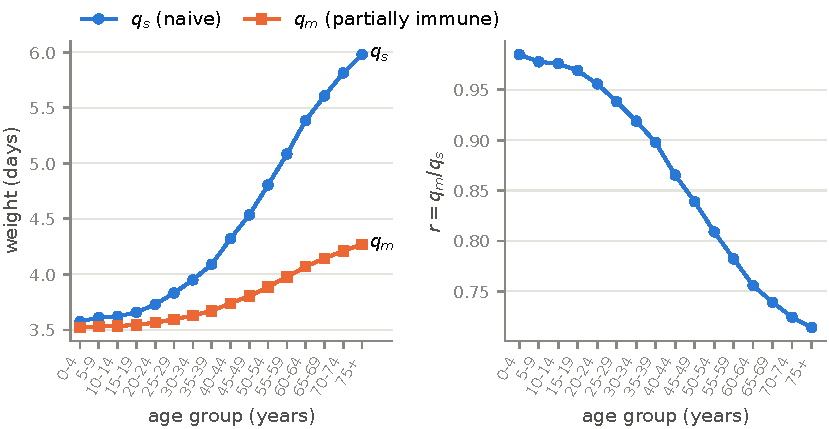
\includegraphics[width=\textwidth]{fig_weights.pdf}
\caption{The weights $q_s$ and $q_m$ of~\eqref{qs-qm} by age (left) and their
ratio $r=q_m/q_s$ (right), $51\times16$ data.}\label{fig-weights}
\end{figure}

\begin{figure}[ht]
\centering
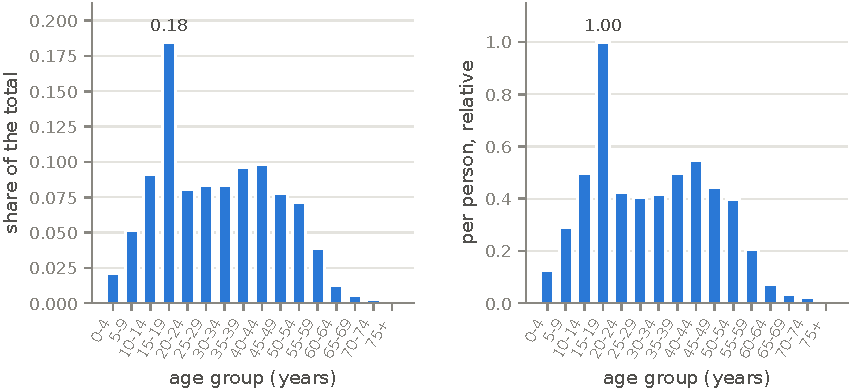
\includegraphics[width=\textwidth]{fig_left_ev.pdf}
\caption{The susceptible rows of the dominant left eigenvector of
$\operatorname{NGM}$ at $\bm\chi=0$, summed over the 51 locations, by age: share
of the total (left), and divided by the population of the age group, relative
to the largest value (right).}\label{fig-left}
\end{figure}

\begin{figure}[ht]
\centering
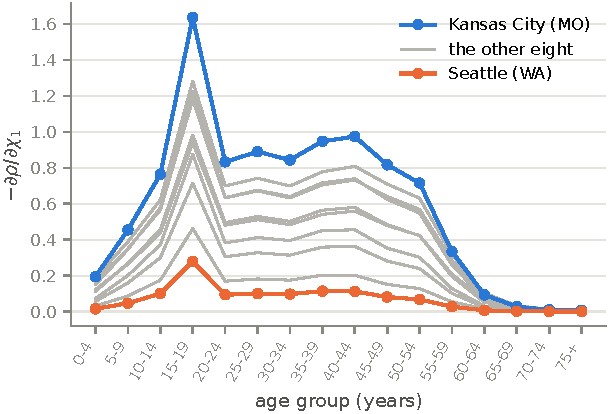
\includegraphics[width=0.75\textwidth]{fig_grad_hhs.pdf}
\caption{$-\partial\rho(\operatorname{NGM})/\partial\chi_{1,p}$ at
$\bm\chi=0$ by age, for the ten states with the headquarters of the HHS
regions; Missouri (Kansas City) and Washington (Seattle) have the largest and
the smallest maximum.}\label{fig-grad}
\end{figure}

\FloatBarrier
\bibliographystyle{plain}
\bibliography{bib_mb}
\end{document}
